\documentclass[aspectratio=1610,brown]{beamer}
\usepackage{amsmath}
\usepackage{graphicx}
\usetheme{Warsaw}
\usecolortheme{rose}
\title{JUNO proton decay: life and sensitivity estimation}
\author{ZhangAiqiang}
\institute{DEP}
\date{}
\begin{document}
\begin{frame}
    \titlepage
\end{frame}
\begin{frame}
    \frametitle{Introduction}
    what we have: Expect background: $b$, Observed signal: $n_o$

    Estimate the signal $s$ upper limit.

    \[\beta=\sum_{n\leq n_o}{\frac{(s_u+b)^ne^{-(s_u+b)}}{n}}\] 
    $CL=1-\beta$, $s_u$ maybe negative
\end{frame}
\section{Bayes Method}
\begin{frame}
    \frametitle{Bayes Method}
    \[1-\beta=\frac{\int_0^{s_u}{(s+b)^n_oe^{-(s+b)}ds}}{\int_0^{\infty}{(s+b)^n_oe^{-(s+b)}ds}}\]
    \begin{columns}
        \begin{column}{0.5\textwidth}
            \begin{enumerate}
                \item solve the problem of negative value
                \item the initial uniform probability is not valid
            \end{enumerate}
        \end{column}
        \begin{column}{0.5\textwidth}
            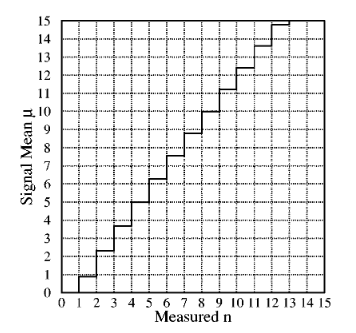
\includegraphics[width=\columnwidth]{figure/bayes.png}
        \end{column}
    \end{columns}
\end{frame}
\section{Feldman Cousin Method}
\begin{frame}
\frametitle{Feldman Cousin Method}
\begin{columns}
    \begin{column}{0.5\textwidth}
            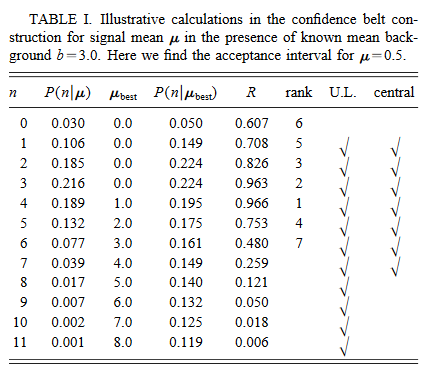
\includegraphics[width=\columnwidth]{figure/fctable.png}
    \end{column}
    \begin{column}{0.5\textwidth}
        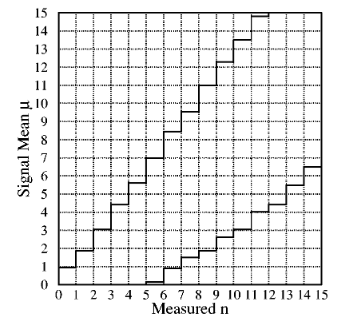
\includegraphics[width=\columnwidth]{figure/fc.png}
    \end{column}
\end{columns}
\end{frame}
\end{document}